\section{Entwurf der Benutzeroberfläche}

\subsection{Aufbau der Präsentationsschicht}

\begin{itemize}
\item Menu-Leiste
    \begin{itemize}
        \item Datei-Menu
        \begin{itemize}
            \item New
            \item Open\dots
            \item Save\dots
            \item Quit        
        \end{itemize}
        \item Edit-Menu
        \begin{itemize}
            \item Textfarbe
        \end{itemize}
        \item Hilfe-Menu
        \begin{itemize}
            \item Versionshinweis        
        \end{itemize}
    \end{itemize}
\item Coolbar-Leiste
\item Tab-Leiste
\end{itemize}



\subsection{Beschreibung der Workflows der Editor-Anwendung}
Zur Veranschaulichung der Editor-Workflows werden Aktivitätsdiagramme nach der UML2-Spezifikation verwendet.
Die folgdenden beiden Diagramme veranschaulichen den Workflow für das Öffnen und Schließen eines Tabs.


\begin{figure}[H]
    \centering
    \begin{subfigure}[b]{0.45\linewidth}
        \centering
        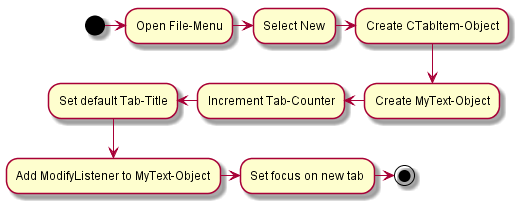
\includegraphics[width=\linewidth]{figures/newtab/newtab.png}
        \caption{Öffnen eines neuen Tabs}
    \end{subfigure}
    \begin{subfigure}[b]{0.45\linewidth}
        \centering
        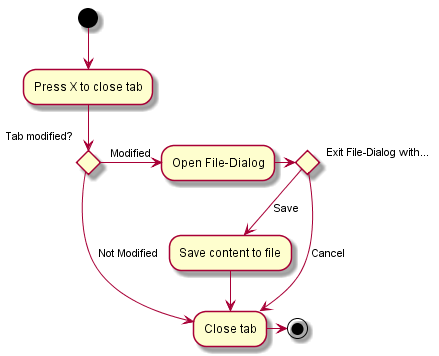
\includegraphics[width=\linewidth]{figures/closetab/closetab.png}
        \caption{Schließen eines Tabs}
    \end{subfigure}
    \caption{Tabs öffnen und schließen}
    \label{fig:tabs}
\end{figure}

\noindent
Weiterhin werden in unserer Editor-Applikation verschiedene Dialogfenster genötigt.
Ein Dialog zur Anzeige der Versionsinformation sowie einen zur Auswahl der Schriftfarbe im aktuell geöffneten Tab.

\begin{figure}[H]
    \centering
    \begin{subfigure}[b]{0.45\linewidth}
        \centering
        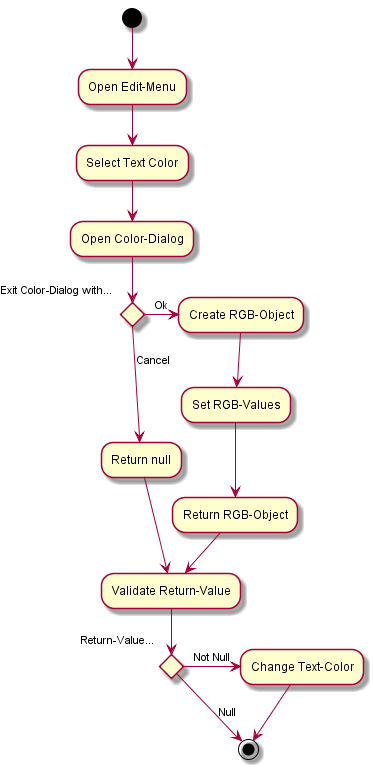
\includegraphics[width=\linewidth]{figures/color/color.png}
        \caption{Zeige Farb-Dialog}
    \end{subfigure}
    \begin{subfigure}[b]{0.45\linewidth}
        \centering
        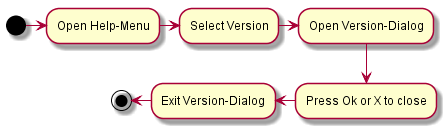
\includegraphics[width=\linewidth]{figures/version/version.png}
        \caption{Zeige Version-Dialog}
    \end{subfigure}
    \caption{Farb- und Versions-Dialog}
    \label{fig:dialogs}
\end{figure}

\noindent
Über das Datei-Menu können Funktionen wie öffnen einer neuen Datei, speichern des geöffneten Tabs und weiteres 
ausgeführt werden. Die möglichen Aktionen sind in der Abbildung \ref{fig:filemenu} zu sehen.

\begin{figure}[H]
    \begin{subfigure}[b]{0.45\linewidth}
        
        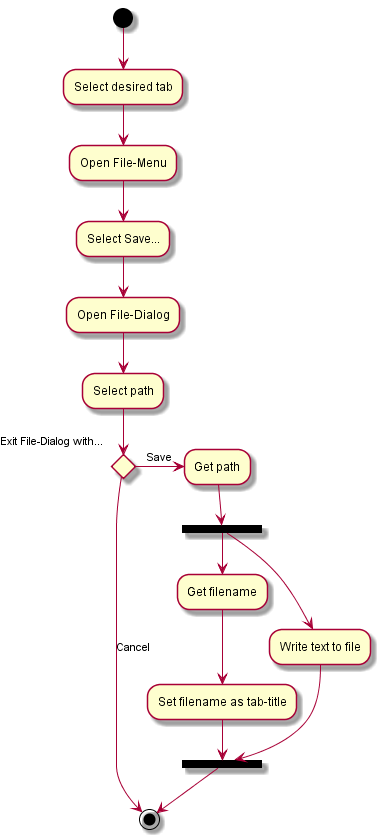
\includegraphics[width=\linewidth]{figures/save/save.png}
        \caption{Datei öffnen}
    \end{subfigure}
    \begin{subfigure}[b]{0.45\linewidth}
        
        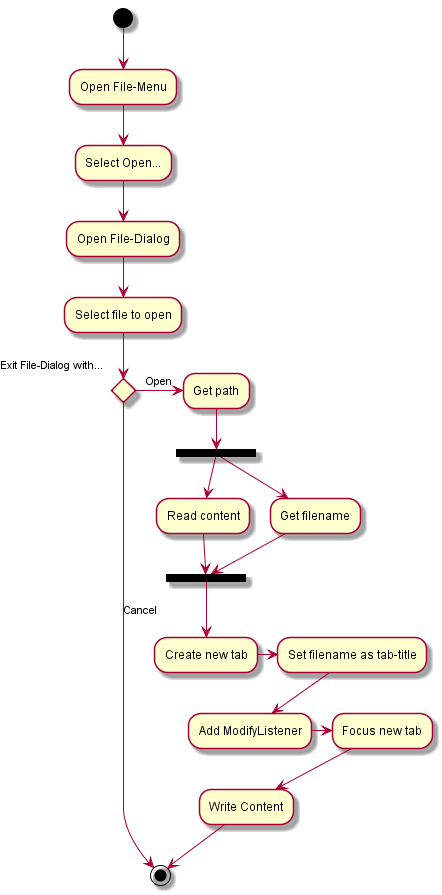
\includegraphics[width=\linewidth]{figures/open/open.png}
        \caption{Text in Datei speichern}
    \end{subfigure}
    \begin{subfigure}[b]{0.4\linewidth}
        
        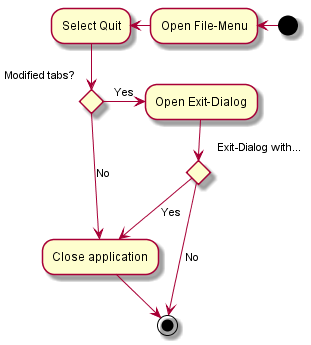
\includegraphics[width=\linewidth]{figures/quit/quit.png}
        \caption{Anwendung beenden}
    \end{subfigure}
    \caption{Aktionen im Datei-Menu}
    \label{fig:filemenu}
\end{figure}

\subsection{Darstellung der Klassenstruktur}
Die Applikation soll in drei Schichten aufgeteilt werde: Präsentations-, Dialogmanagement- und Applikationsschicht.
In Abbildung \ref{fig:presentationlayer}, \ref{fig:dialogmanagementlayer} und \ref{fig:applicationlayer} sind die
drei Schichten im UML2-Klassendiagramm dargestellt.

\begin{figure}[H]
    \centering
    \begin{subfigure}[b]{0.5\linewidth}
        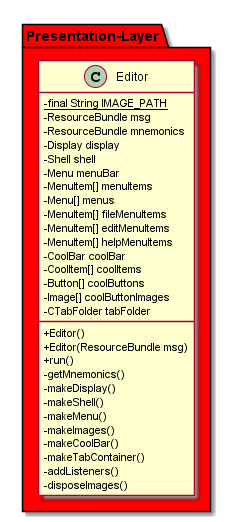
\includegraphics[width=\linewidth]{figures/class/class_diagram_presentation.png}
    \end{subfigure}
    \begin{subfigure}[b]{0.4\linewidth}
        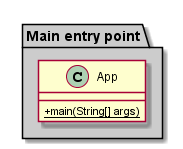
\includegraphics[width=\linewidth]{figures/class/class_diagram_main.png}    
    \end{subfigure}
    \caption{Präsentationsschicht}
    \label{fig:presentationlayer}
\end{figure}
\begin{figure}[H]
    \centering
    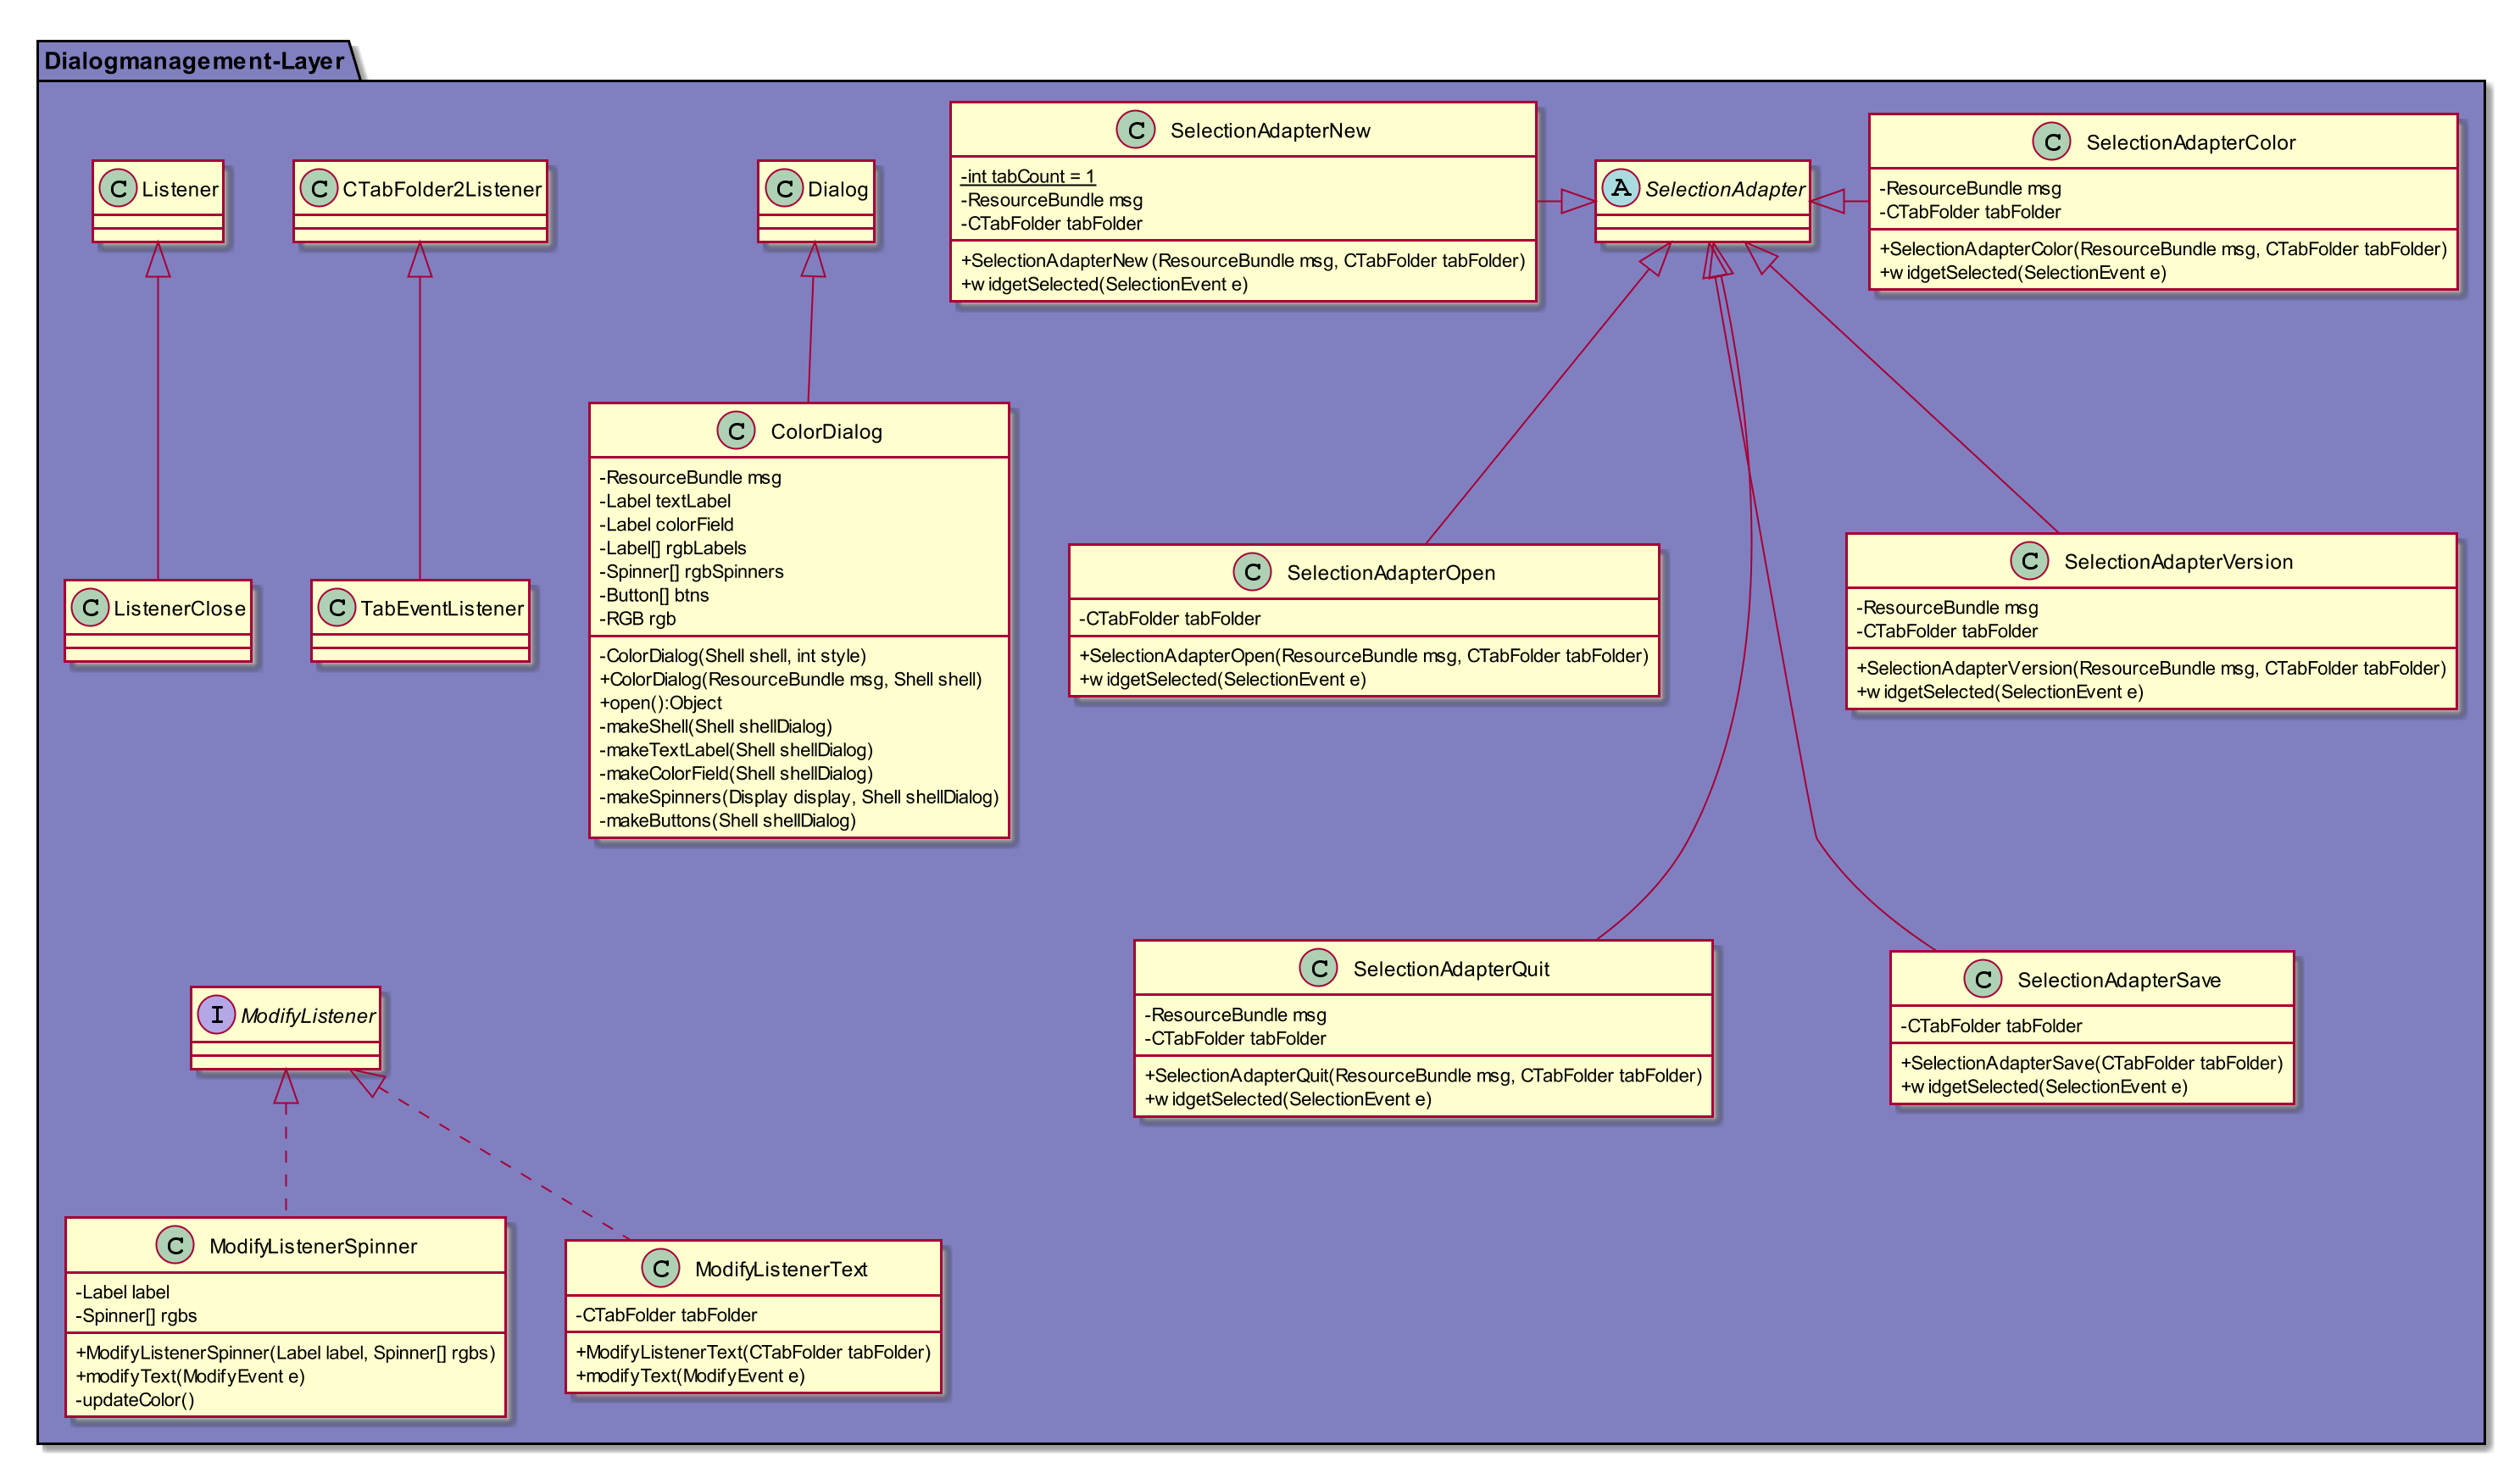
\includegraphics[width=\linewidth]{figures/class/class_diagram_dialogmanagement.png}
    \caption{Dialogmanagementschicht}
    \label{fig:dialogmanagementlayer}
\end{figure}
\begin{figure}[H]
    \centering
    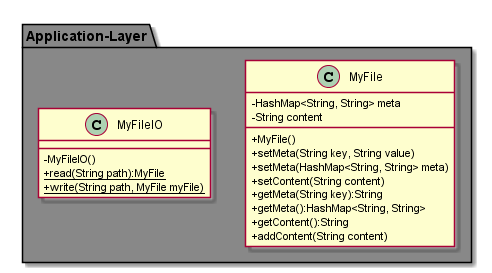
\includegraphics[width=0.7\linewidth]{figures/class/class_diagram_application.png}
    \caption{Applikationsschicht}
    \label{fig:applicationlayer}
\end{figure}
\begin{figure}[H]
    \centering
    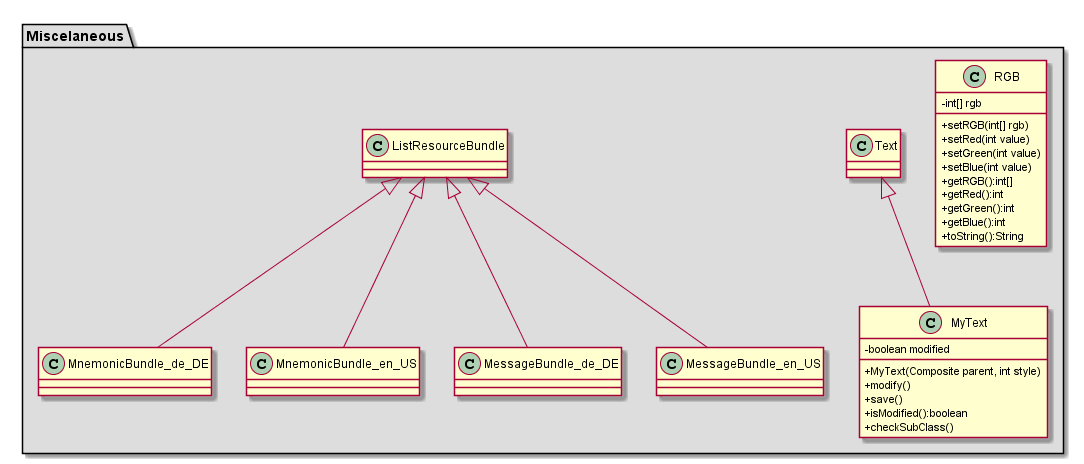
\includegraphics[width=0.7\linewidth]{figures/class/class_diagram_misc.png}
    \caption{Weitere erstellte Klassen}
    \label{fig:miscclasses}
\end{figure}

\noindent
Da das Klassendiagramm bereits realtiv viele und große Klassen enthält, haben wir uns dagegen entschieden alle
Assoziationen zwischen den Klassen darzustellen (lediglich die Vererbungshierarchien sind dargestellt).
Abbildung \ref{fig:example} zeigt einen Teil der Gesamtapplikation mit entsprechenden Assoziationen.

\begin{figure}[H]
    \centering
    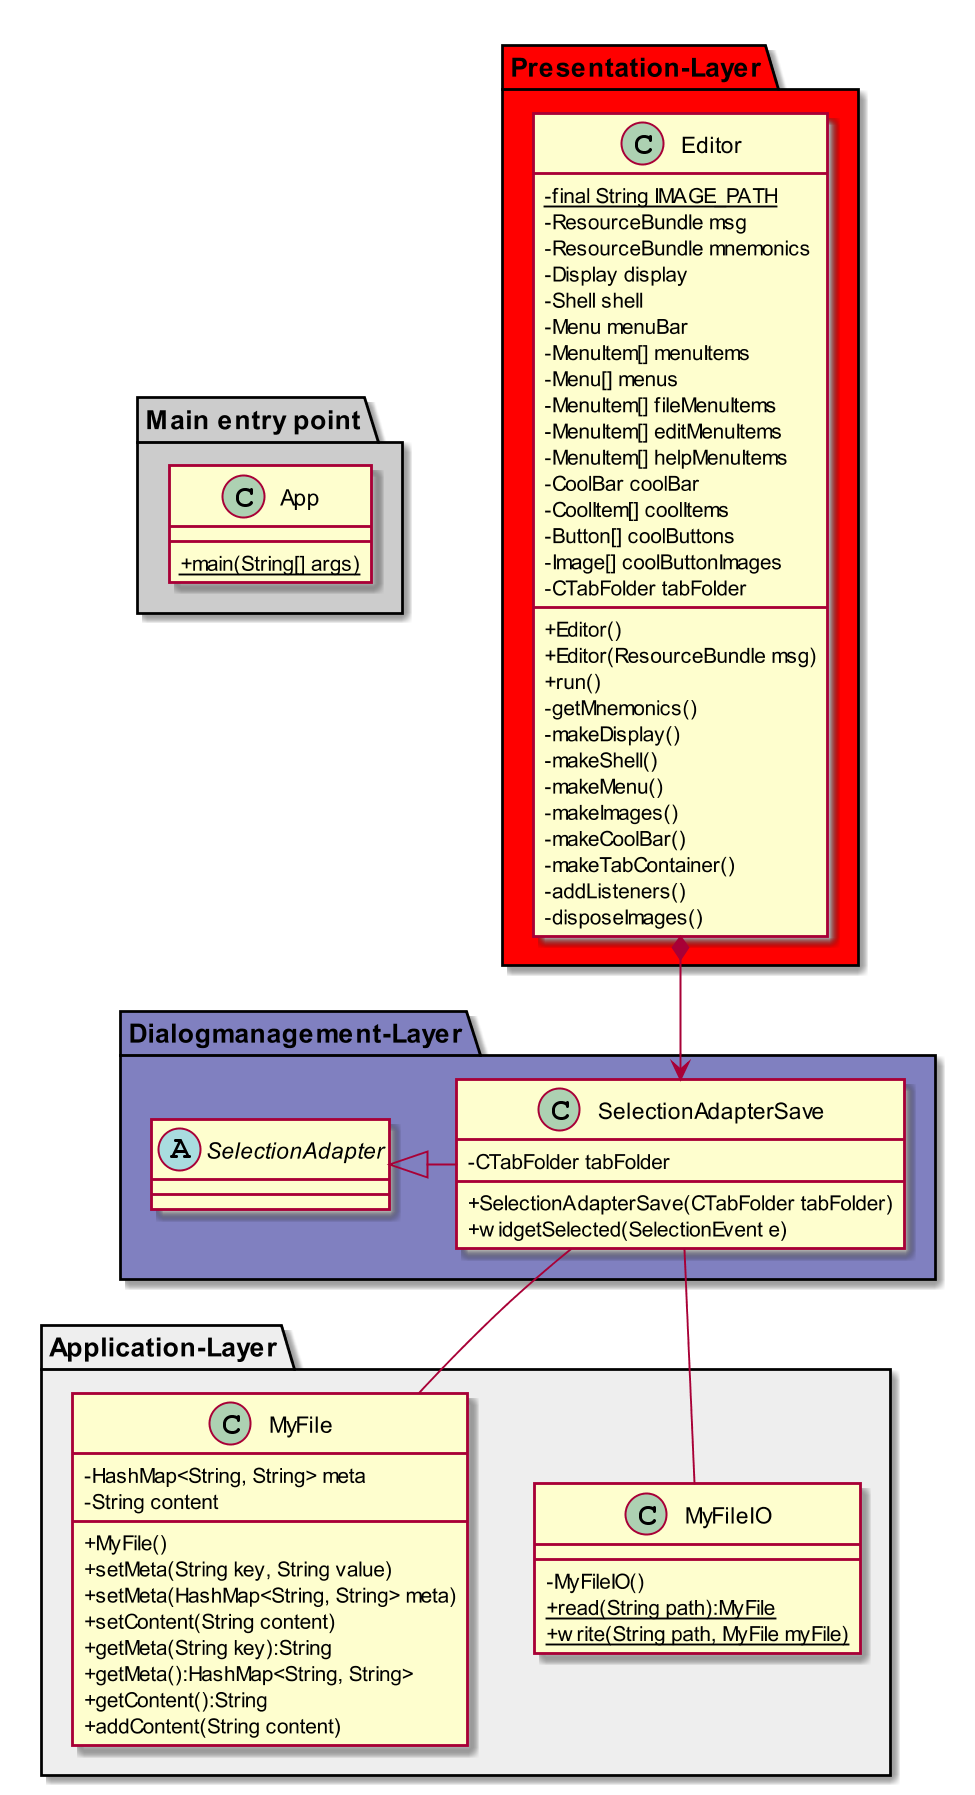
\includegraphics[width=0.7\linewidth]{figures/class/class_diagram_example.png}
    \caption{Tab in Datei speichern}
    \label{fig:example}
\end{figure}
